\fancychapter{Results: Pirate Game}
\label{ap:d}

\section{$3$ Player Game}

\subsection{Simulation}
\begin{lstlisting}


function out = simulationQuantumPirateGame3Players(a_11,a_12,a_13,a_22,a_23, gamma, U1,U2,U3,U4,U5)
%
%        IN:
%-- alocation proposal a_ij -i number of the player that proposes a_ij coins
%   to player j
%-- gamma entanglemen coefitient
%-- U1, U2, U3, U4, U5 player's strategies; default CDCCD
%
%       OUT:
%-- expected utility for players 1 ,2 ,3:  [u1 u2 u3]

%-- Check variables and set to defaults
if exist('a_11','var')~=1, a_11=99; end
if exist('a_12','var')~=1, a_12=0; end
if exist('a_13','var')~=1, a_13=1; end
if exist('a_22','var')~=1, a_22=100; end
if exist('a_23','var')~=1, a_23=0; end
if exist('gamma','var')~=1, gamma=0; end

%-- Classic Pure Strategy Operators
%   cooperate= [1 0;0 1]
C= eye(2);
%   defect= [0 1;1 0]
D= ones(2)-eye(2);
D(2,1)=1;

if exist('U1','var')~=1, U1=C; end
if exist('U2','var')~=1, U2=D; end
if exist('U3','var')~=1, U3=C; end
if exist('U4','var')~=1, U4=C; end
if exist('U5','var')~=1, U5=D; end

%-- Matrix containing all pure-states for hilbert space 32
H32B=eye(32);

step=0.1;
t=0:step:pi;

i=gamma;

%-- varying the entanglement parameter

%-- Building the initial state, for the entanglement parameter i
ini= cos(i/2)*kron([1 0]', kron([1 0]',[1 0]'))+1i*sin(i/2)*kron([0 1]', kron([0 1]',[0 1]'));
%-- Entanglement Gate J
J= expm(1i*(i/2)*kron(D,kron(D,kron(D,kron(D,D)))));
%-- Alternative way to build the initial state
ini= J*H32B(:,1);
%-- Deentangles to produce a final state
Jd = ctranspose( J);

H= fft(eye(2))/sqrt(2);
fin = kron(U1,kron(U2,kron(U3,kron(U4,U5))))*ini;
fin= Jd*fin;
out = expectedUtility(fin, a_11,a_12,a_13,a_22,a_23);

end


function out = expectedUtility(fin, a_11,a_12,a_13,a_22,a_23)
%payofffunc_player1(fin)
%
%                Calculates the payoff for player 1
%              IN
%                   fin: final state
%

%-- Check variables and set to defaults
if exist('a_11','var')~=1, a_11=99; end
if exist('a_12','var')~=1, a_12=0; end
if exist('a_13','var')~=1, a_13=1; end
if exist('a_22','var')~=1, a_22=100; end
if exist('a_23','var')~=1, a_23=0; end

%-- Matrix containing all pure-states for hilbert space 32
H32B=eye(32);

prob_proposal_1_accepted=0;
for accepted=[1 2 3 4 5 6 7 8 9 10 11 12 17 18 19 20]
    prob_proposal_1_accepted= prob_proposal_1_accepted + measure(H32B(:,accepted),fin);
end
prob_proposal_1_accepted;

prob_proposal_1_rejected=0;
for rejected=[13 14 15 16 21 22 23 24 25 26 27 28 29 30 31 32]
    prob_proposal_1_rejected= prob_proposal_1_rejected + measure(H32B(:,rejected),fin);
end
prob_proposal_1_rejected;

prob_proposal_2_accepted=0;
for accepted=[13 14 15 21 22 23 25 26 27 29 30 31]
    prob_proposal_1_accepted= prob_proposal_1_accepted + measure(H32B(:,accepted),fin);
end
prob_proposal_2_accepted;

prob_proposal_2_rejected=0;
for rejected=[16 24 28 32]
    prob_proposal_1_rejected= prob_proposal_1_rejected + measure(H32B(:,rejected),fin);
end
prob_proposal_2_rejected;

u1 = a_11*prob_proposal_1_accepted -200* prob_proposal_1_rejected;

u2 = a_12*prob_proposal_1_accepted +(0.5 + a_22)*prob_proposal_2_accepted -199.5*prob_proposal_2_rejected;

u3 = a_13*prob_proposal_1_accepted +(0.5 + a_23)*prob_proposal_2_accepted + 100.5*prob_proposal_2_rejected;
out =[ u1 u2 u3];
end

function m = measure(b,fin)
m= (norm(conj(b).*fin))^2;
end


function u= U_thetha_phi(theta,phi)
u= [exp(1i*phi)cos(theta/2) *sin(theta/2);sin(theta/2) -exp(-i*phi)*cos(theta/2)];
end
\end{lstlisting}

\subsection{ Captain proposes $(99,0,1)$.}
 
\subsubsection{ Accepted proposal after 1 round of the game.}
\label{tabs:accepted99}

\begin{table}[ht]
\begin{center}

\begin{tabular}{cc}
  a)\putindeepbox[7pt]{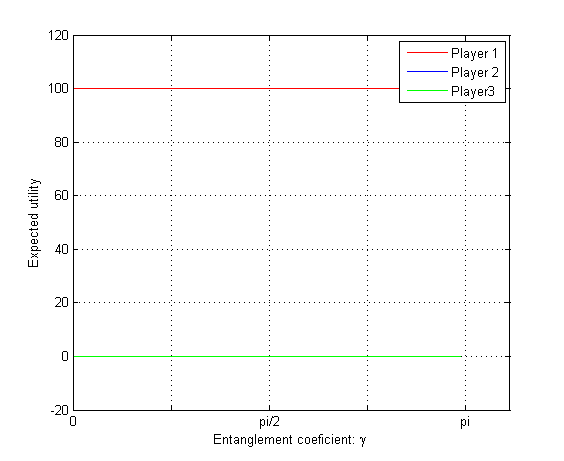
\includegraphics[scale=0.46]{3Accepted99/CCC.PNG}}
    & a1)\putindeepbox[7pt]{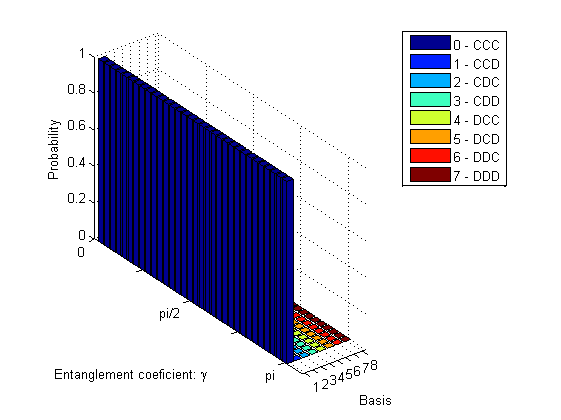
\includegraphics[scale=0.46]{3Accepted99/CCC_1.PNG}} \\
\end{tabular}
\caption{a) Expected utility for $3$ players, where the players will use the $(Cooperate, Cooperate, Cooperate)$ operators. The initial proposal is $(\alpha_{1}, \alpha_{2}, \alpha_{3}) =(99, 0, 1)$. a1) Probability distribution of the final state depending on the entanglement coefficient $\gamma$. }
\label{tab:3playerCCC99}
\end{center}
 \end{table}

\begin{table}[h]
\begin{center}
\begin{tabular}{cc}
  b)\putindeepbox[7pt]{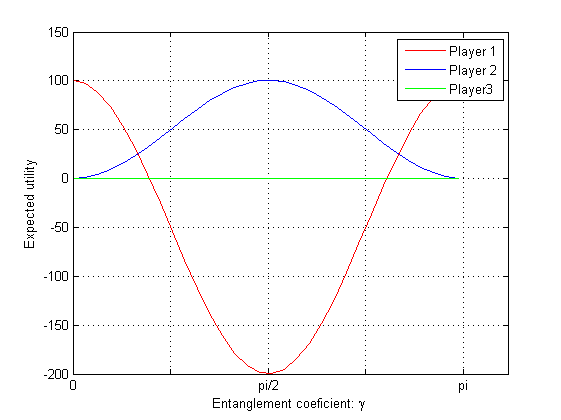
\includegraphics[scale=0.46]{3Accepted99/CCD.PNG}}
    & b1)\putindeepbox[7pt]{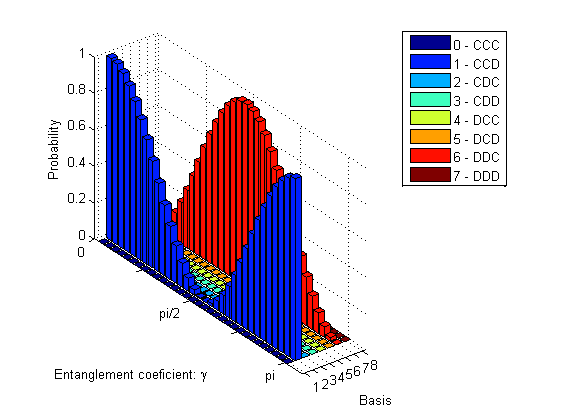
\includegraphics[scale=0.46]{3Accepted99/CCD_1.PNG}} \\
\end{tabular}
\caption{b) Expected utility for $3$ players, where the players will use the $(Cooperate, Cooperate, Defect)$ operators. b1) Probability distribution of the final state depending on the entanglement coefficient $\gamma$. }
\label{tab:3playerCCD99}
\end{center}
 \end{table}

\begin{table}[h]
\begin{center}
\begin{tabular}{cc}
  c)\putindeepbox[7pt]{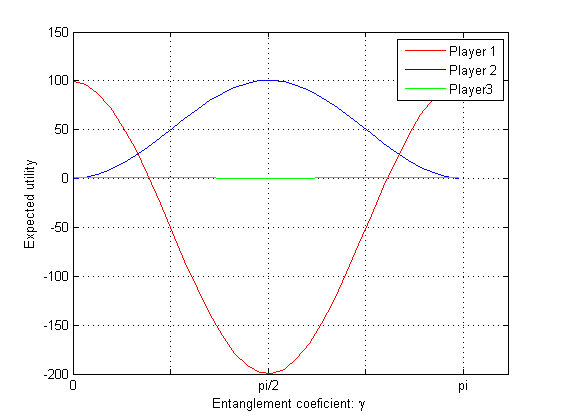
\includegraphics[scale=0.46]{3Accepted99/CDC.PNG}}
    & c1)\putindeepbox[7pt]{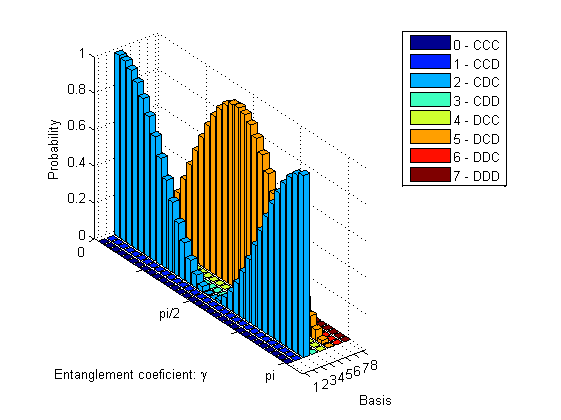
\includegraphics[scale=0.46]{3Accepted99/CDC_1.PNG}} \\
\end{tabular}
\caption{c) Expected utility for $3$ players, where the players will use the $(Cooperate, Defect, Cooperate)$ operators. c1) Probability distribution of the final state depending on the entanglement coefficient $\gamma$. }
\label{tab:3playerCDC99}
\end{center}
 \end{table}

\begin{table}[h]
\begin{center}
\begin{tabular}{cc}
  d)\putindeepbox[7pt]{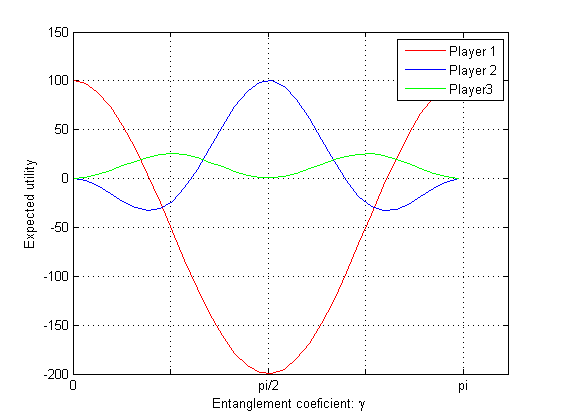
\includegraphics[scale=0.46]{3Accepted99/DCC.PNG}}
    & d1)\putindeepbox[7pt]{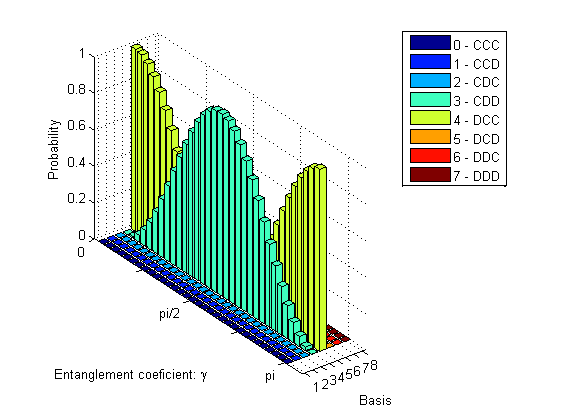
\includegraphics[scale=0.46]{3Accepted99/DCC_1.PNG}} \\
\end{tabular}
\caption{b) Expected utility for $3$ players, where the players will use the $(Defect, Cooperate, Cooperate)$ operators. b1) Probability distribution of the final state depending on the entanglement coefficient $\gamma$. }
\label{tab:3playerDCC99}
\end{center}
 \end{table}

\clearpage
\subsubsection{Initial proposal rejected; $(Cooperate , Defect, Defect)$}
\label{ap:d:CDD99}
%\item  Rejected proposal after 1 round of the game.\\

%\begin{itemize}

%\item In the first round the players use the operators $(CDD)$.\\

\begin{table}[h]
\begin{center}
\begin{tabular}{cc}
  a)\putindeepbox[7pt]{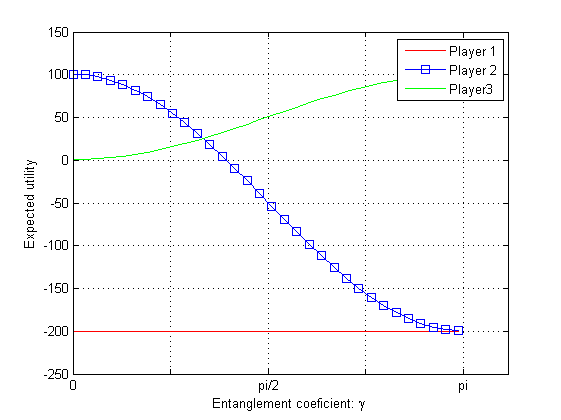
\includegraphics[scale=0.46]{3Rejected99/CDD_CC.PNG}}
    & a1)\putindeepbox[7pt]{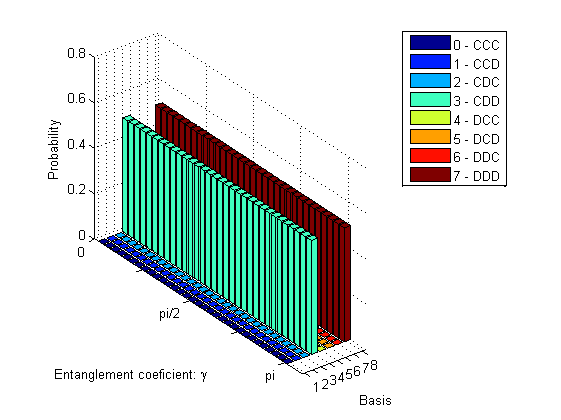
\includegraphics[scale=0.46]{3Rejected99/CDD_CC1.PNG}} \\
\end{tabular}
\caption{a) Expected utility for $3$ players, where the players will use the $(Cooperate , Defect, Defect)$ operators in the first round of the game; in the second round player 2 and player 3 will play $(CC)$. }
\label{tab:3playerCDD_CC99}
\end{center}
 \end{table}

\begin{table}[h]
\begin{center}
\begin{tabular}{cc}
  b)\putindeepbox[7pt]{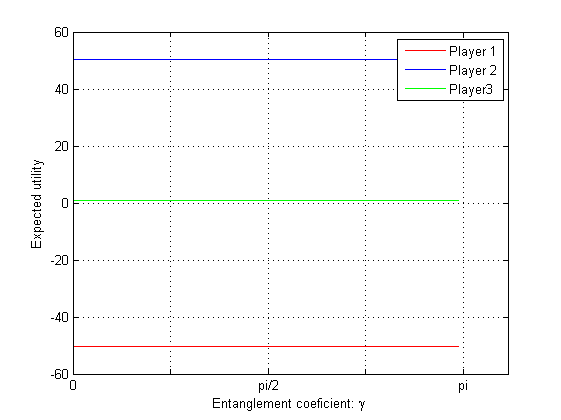
\includegraphics[scale=0.46]{3Rejected99/CDD_CD.PNG}}
    & b1)\putindeepbox[7pt]{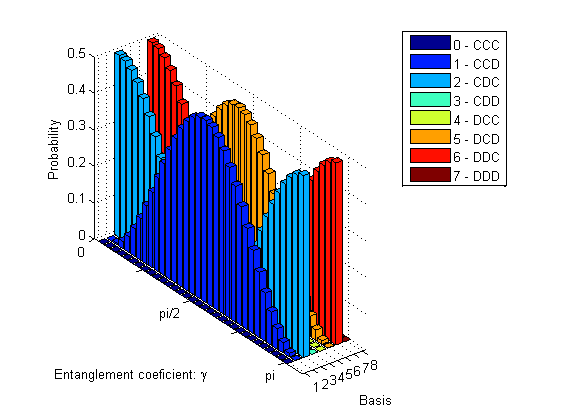
\includegraphics[scale=0.46]{3Rejected99/CDD_CD1.PNG}} \\
\end{tabular}
\caption{b) Expected utility for $3$ players, where the players will use the $(Cooperate , Defect, Defect)$ operators in the first round of the game; in the second round player 2 and player 3 will play $(CD)$. }
\label{tab:3playerCDD_CD99}
\end{center}
 \end{table}

\begin{table}[h]
\begin{center}
\begin{tabular}{cc}
  c)\putindeepbox[7pt]{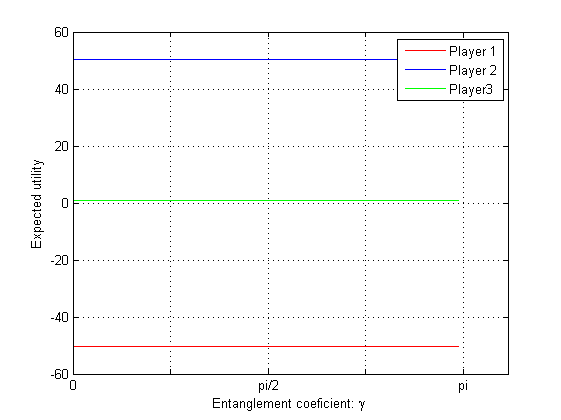
\includegraphics[scale=0.46]{3Rejected99/CDD_DC.PNG}}
    & c1)\putindeepbox[7pt]{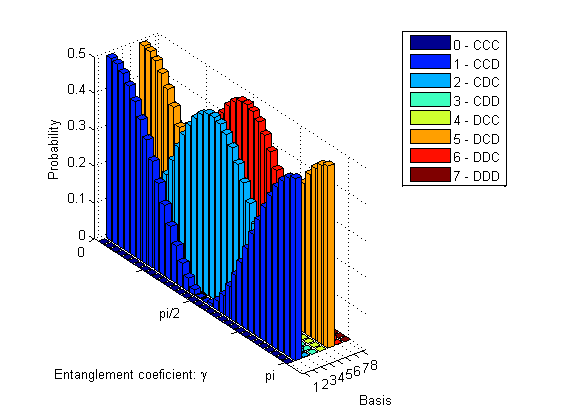
\includegraphics[scale=0.46]{3Rejected99/CDD_DC1.PNG}} \\
\end{tabular}
\caption{c) Expected utility for $3$ players, where the players will use the $(Cooperate , Defect, Defect)$ operators in the first round of the game; in the second round player 2 and player 3 will play $(DC)$. }
\label{tab:3playerCDD_DC99}
\end{center}
 \end{table}

\begin{table}[h]
\begin{center}
\begin{tabular}{cc}
  d)\putindeepbox[7pt]{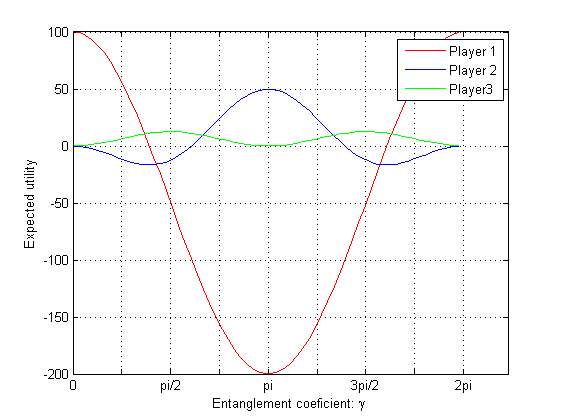
\includegraphics[scale=0.46]{3Rejected99/CDD_DD.PNG}}
    & d1)\putindeepbox[7pt]{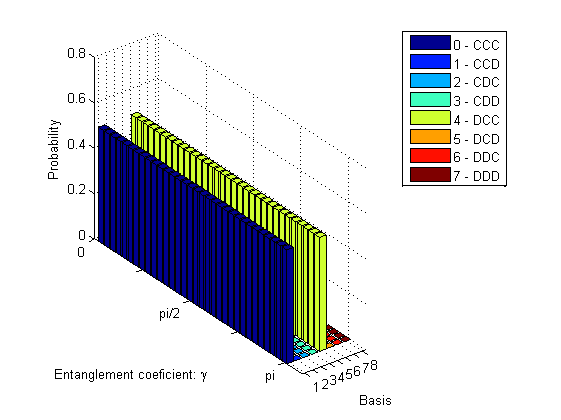
\includegraphics[scale=0.46]{3Rejected99/CDD_DD1.PNG}} \\
\end{tabular}
\caption{b) Expected utility for $3$ players, where the players will use the $(Cooperate , Defect, Defect)$ operators in the first round of the game; in the second round player 2 and player 3 will play $(DD)$. }
\label{tab:3playerCDD_DD99}
\end{center}
 \end{table}


\clearpage
\subsubsection{Initial proposal rejected; $(Defect, Cooperate, Defect)$}

\begin{table}[h]
\begin{center}
\begin{tabular}{cc}
  a)\putindeepbox[7pt]{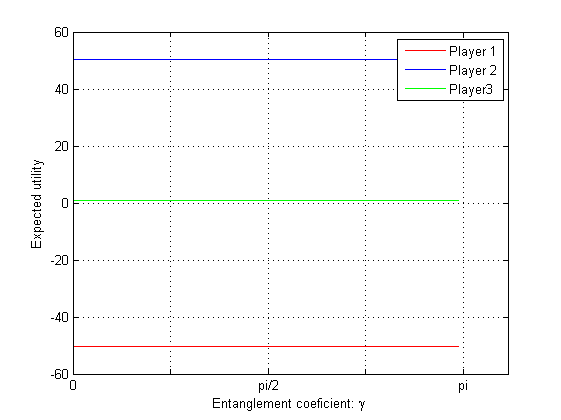
\includegraphics[scale=0.46]{3Rejected99/DCD_CC.PNG}}
    & a1)\putindeepbox[7pt]{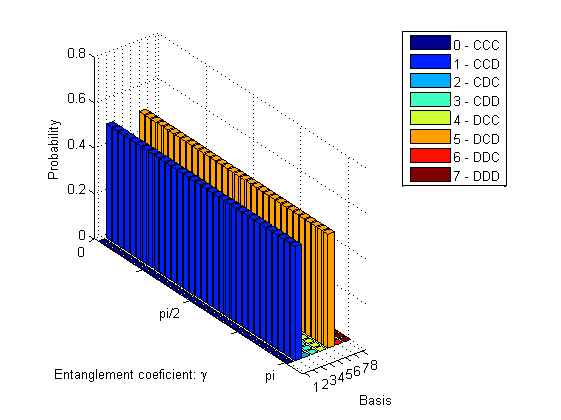
\includegraphics[scale=0.46]{3Rejected99/DCD_CC1.PNG}} \\
\end{tabular}
\caption{a) Expected utility for $3$ players, where the players will use the $(Defect, Cooperate, Defect)$ operators in the first round of the game; in the second round player 2 and player 3 will play $(CC)$. }
\label{tab:3playerDCD_CC99}
\end{center}
 \end{table}

\begin{table}[h]
\begin{center}
\begin{tabular}{cc}
  b)\putindeepbox[7pt]{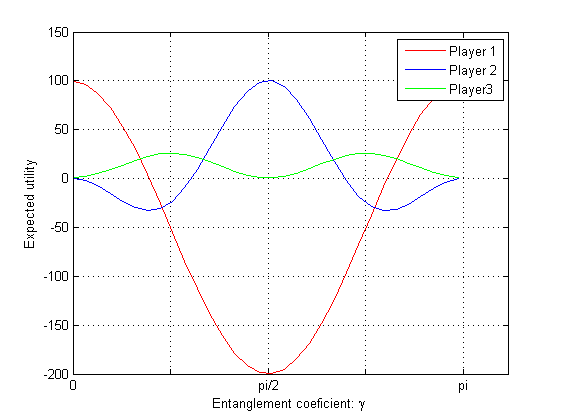
\includegraphics[scale=0.46]{3Rejected99/DCD_CD.PNG}}
    & b1)\putindeepbox[7pt]{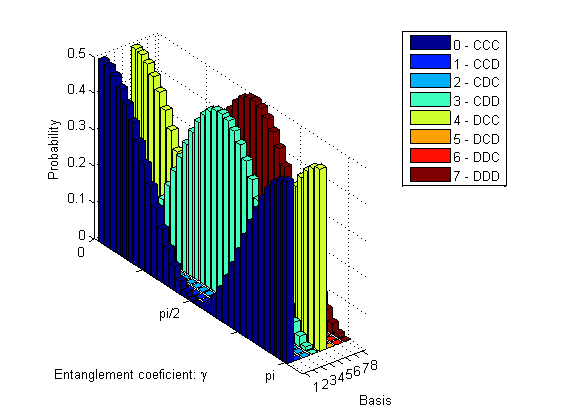
\includegraphics[scale=0.46]{3Rejected99/DCD_CD1.PNG}} \\
\end{tabular}
\caption{b) Expected utility for $3$ players, where the players will use the $(Defect, Cooperate, Defect)$ operators in the first round of the game; in the second round player 2 and player 3 will play $(CD)$. }
\label{tab:3playerDCD_CD99}
\end{center}
 \end{table}

\begin{table}[h]
\begin{center}
\begin{tabular}{cc}
  c)\putindeepbox[7pt]{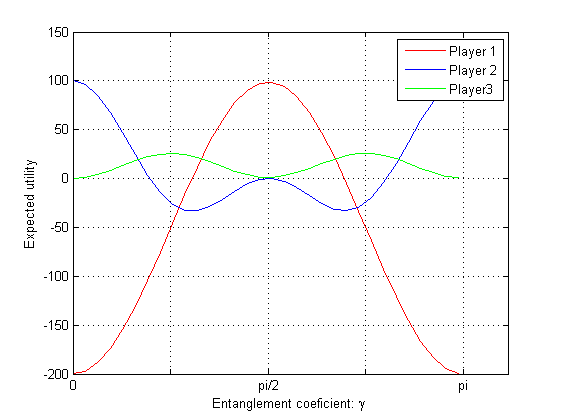
\includegraphics[scale=0.46]{3Rejected99/DCD_DC.PNG}}
    & c1)\putindeepbox[7pt]{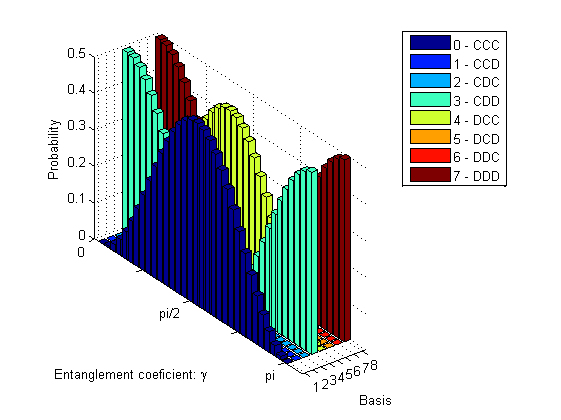
\includegraphics[scale=0.46]{3Rejected99/DCD_DC1.PNG}} \\
\end{tabular}
\caption{c) Expected utility for $3$ players, where the players will use the $(Defect, Cooperate, Defect)$ operators in the first round of the game; in the second round player 2 and player 3 will play $(DC)$. }
\label{tab:3playerDCD_DC99}
\end{center}
 \end{table}

\begin{table}[h]
\begin{center}
\begin{tabular}{cc}
  d)\putindeepbox[7pt]{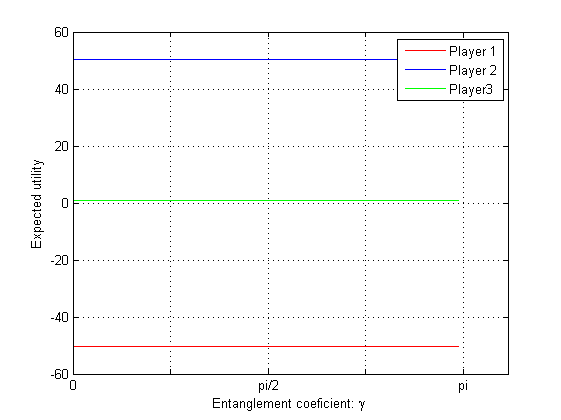
\includegraphics[scale=0.46]{3Rejected99/DCD_DD.PNG}}
    & d1)\putindeepbox[7pt]{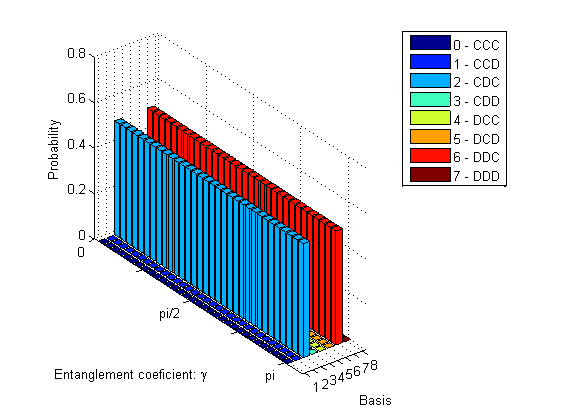
\includegraphics[scale=0.46]{3Rejected99/DCD_DD1.PNG}} \\
\end{tabular}
\caption{b) Expected utility for $3$ players, where the players will use the $(Defect, Cooperate, Defect)$ operators in the first round of the game; in the second round player 2 and player 3 will play $(DD)$. }
\label{tab:3playerDCD_DD99}
\end{center}
 \end{table}

\clearpage
\subsubsection{Initial proposal rejected; $(Defect, Defect, Cooperate)$}

\begin{table}[h]
\begin{center}
\begin{tabular}{cc}
  a)\putindeepbox[7pt]{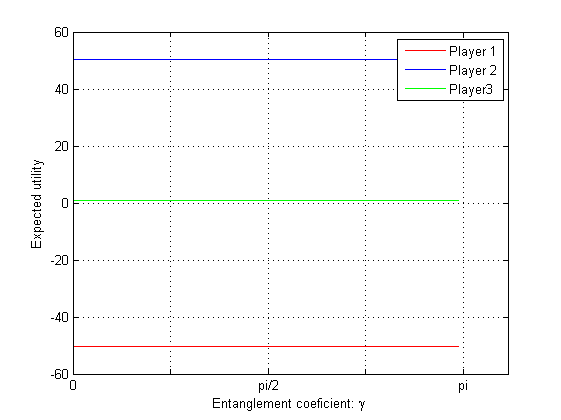
\includegraphics[scale=0.46]{3Rejected99/DDC_CC.PNG}}
    & a1)\putindeepbox[7pt]{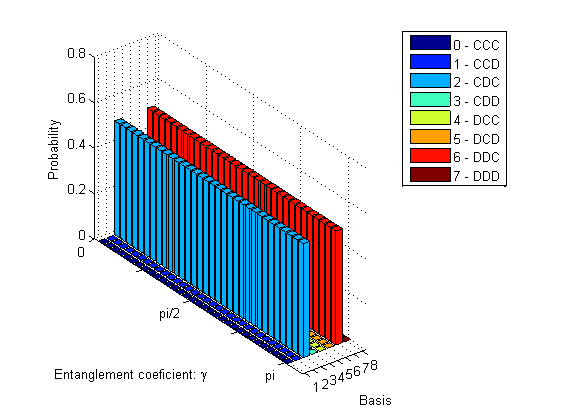
\includegraphics[scale=0.46]{3Rejected99/DDC_CC1.PNG}} \\
\end{tabular}
\caption{a) Expected utility for $3$ players, where the players will use the $(Defect, Defect, Cooperate)$ operators in the first round of the game; in the second round player 2 and player 3 will play $(CC)$. }
\label{tab:3playerDDC_CC99}
\end{center}
 \end{table}

\begin{table}[h]
\begin{center}
\begin{tabular}{cc}
  b)\putindeepbox[7pt]{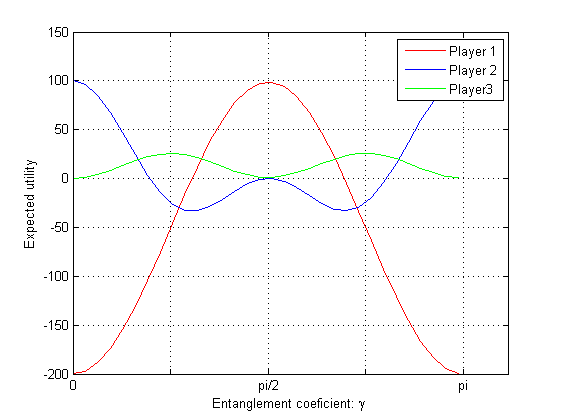
\includegraphics[scale=0.46]{3Rejected99/DDC_CD.PNG}}
    & b1)\putindeepbox[7pt]{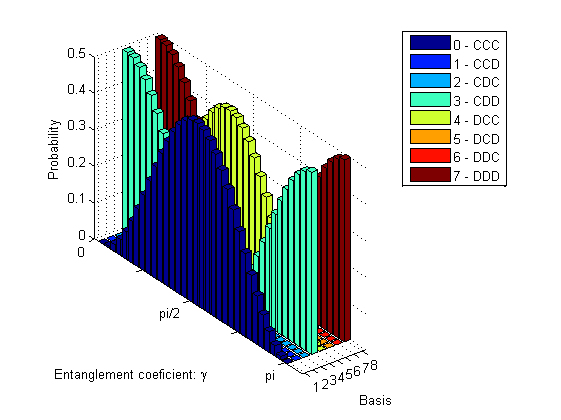
\includegraphics[scale=0.46]{3Rejected99/DDC_CD1.PNG}} \\
\end{tabular}
\caption{b) Expected utility for $3$ players, where the players will use the $(Defect, Defect, Cooperate)$ operators in the first round of the game; in the second round player 2 and player 3 will play $(CD)$. }
\label{tab:3playerDDC_CD99}
\end{center}
 \end{table}

\begin{table}[h]
\begin{center}
\begin{tabular}{cc}
  c)\putindeepbox[7pt]{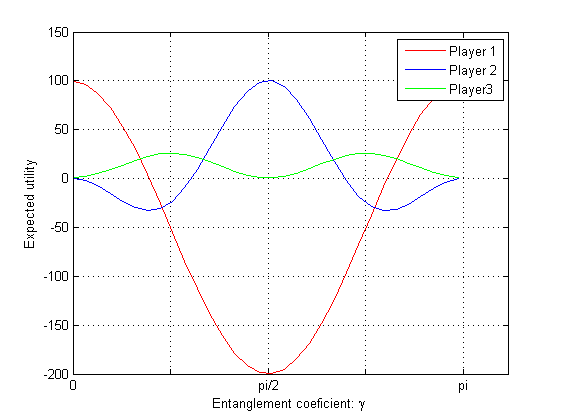
\includegraphics[scale=0.46]{3Rejected99/DDC_DC.PNG}}
    & c1)\putindeepbox[7pt]{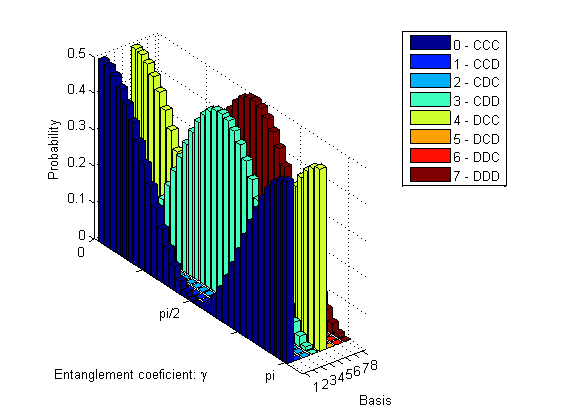
\includegraphics[scale=0.46]{3Rejected99/DDC_DC1.PNG}} \\
\end{tabular}
\caption{c) Expected utility for $3$ players, where the players will use the $(Defect, Defect, Cooperate)$ operators in the first round of the game; in the second round player 2 and player 3 will play $(DC)$. }
\label{tab:3playerDDC_DC99}
\end{center}
 \end{table}

\begin{table}[h]
\begin{center}
\begin{tabular}{cc}
  d)\putindeepbox[7pt]{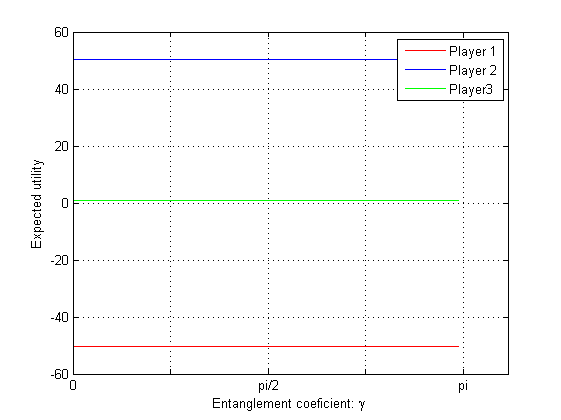
\includegraphics[scale=0.46]{3Rejected99/DDC_DD.PNG}}
    & d1)\putindeepbox[7pt]{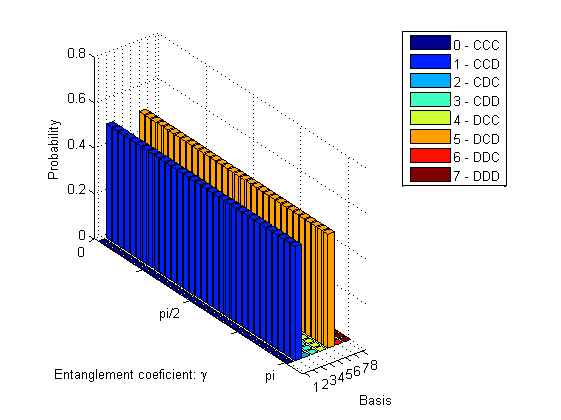
\includegraphics[scale=0.46]{3Rejected99/DDC_DD1.PNG}} \\
\end{tabular}
\caption{b) Expected utility for $3$ players, where the players will use the $(Defect, Defect, Cooperate)$ operators in the first round of the game; in the second round player 2 and player 3 will play $(DD)$. }
\label{tab:3playerDDC_DD99}
\end{center}
 \end{table}

\clearpage
\subsubsection{Initial proposal rejected; $(Defect, Defect, Defect)$}

\begin{table}[h]
\begin{center}
\begin{tabular}{cc}
  a)\putindeepbox[7pt]{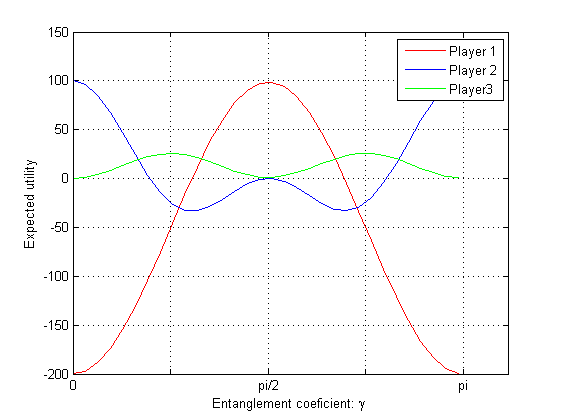
\includegraphics[scale=0.46]{3Rejected99/DDD_CC.PNG}}
    & a1)\putindeepbox[7pt]{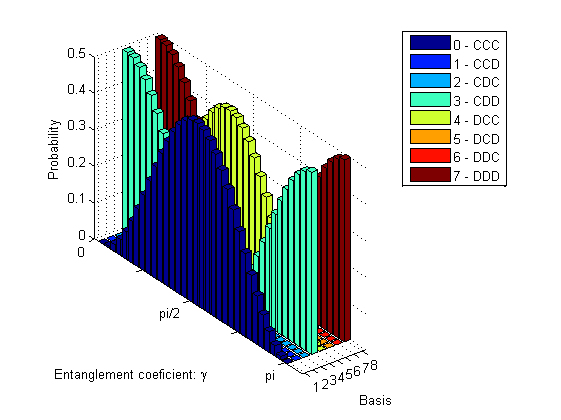
\includegraphics[scale=0.46]{3Rejected99/DDD_CC1.PNG}} \\
\end{tabular}
\caption{a) Expected utility for $3$ players, where the players will use the $(Defect, Defect, Defect)$ operators in the first round of the game; in the second round player 2 and player 3 will play $(CC)$. }
\label{tab:3playerDDD_CC99}
\end{center}
 \end{table}

\begin{table}[h]
\begin{center}
\begin{tabular}{cc}
  b)\putindeepbox[7pt]{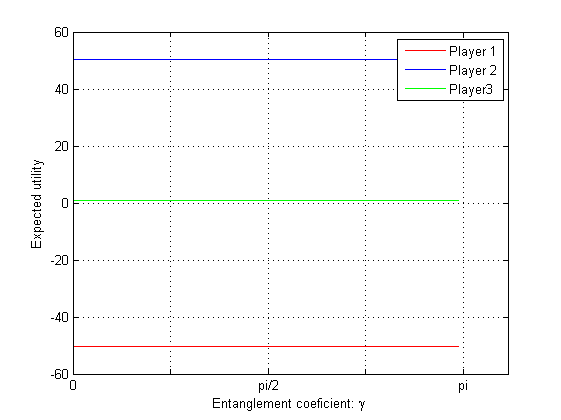
\includegraphics[scale=0.46]{3Rejected99/DDD_CD.PNG}}
    & b1)\putindeepbox[7pt]{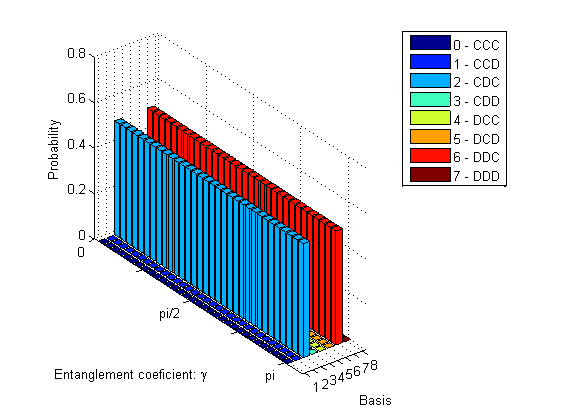
\includegraphics[scale=0.46]{3Rejected99/DDD_CD1.PNG}} \\
\end{tabular}
\caption{b) Expected utility for $3$ players, where the players will use the $(Defect, Defect, Defect)$ operators in the first round of the game; in the second round player 2 and player 3 will play $(CD)$. }
\label{tab:3playerDDD_CD99}
\end{center}
 \end{table}

\begin{table}[ht]
\begin{center}
\begin{tabular}{cc}
  c)\putindeepbox[7pt]{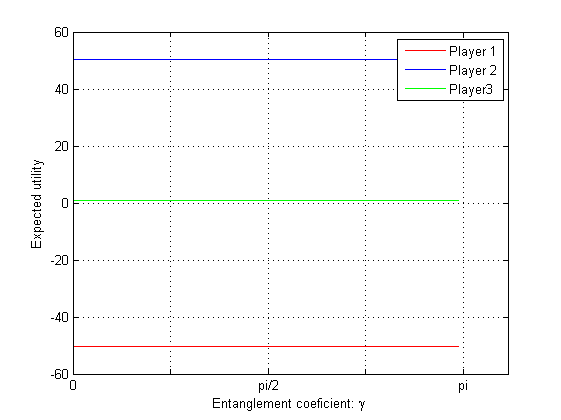
\includegraphics[scale=0.46]{3Rejected99/DDD_DC.PNG}}
    & c1)\putindeepbox[7pt]{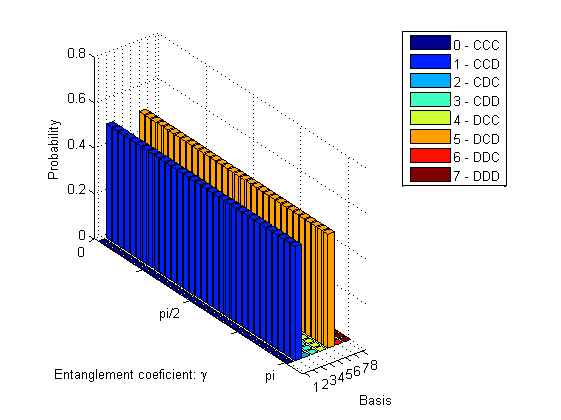
\includegraphics[scale=0.46]{3Rejected99/DDD_DC1.PNG}} \\
\end{tabular}
\caption{c) Expected utility for $3$ players, where the players will use the $(Defect, Defect, Defect)$ operators in the first round of the game; in the second round player 2 and player 3 will play $(DC)$. }
\label{tab:3playerDDD_DC99}
\end{center}
 \end{table}

\begin{table}[h]
\begin{center}
\begin{tabular}{cc}
  d)\putindeepbox[7pt]{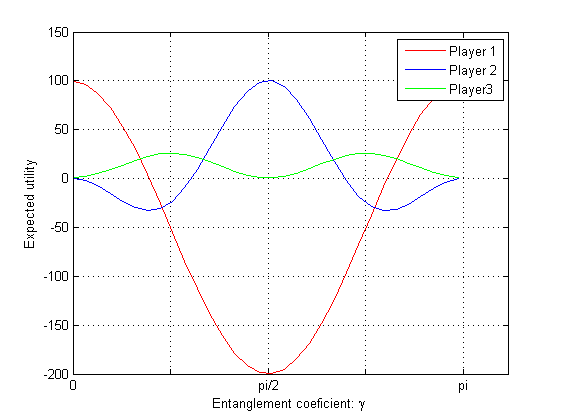
\includegraphics[scale=0.46]{3Rejected99/DDD_DD.PNG}}
    & d1)\putindeepbox[7pt]{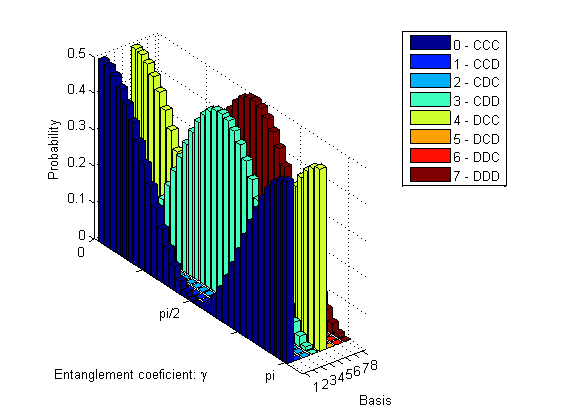
\includegraphics[scale=0.46]{3Rejected99/DDD_DD1.PNG}} \\
\end{tabular}
\caption{b) Expected utility for $3$ players, where the players will use the $(Defect, Defect, Defect)$ operators in the first round of the game; in the second round player 2 and player 3 will play $(DD)$. }
\label{tab:3playerDDD_DD99}
\end{center}
 \end{table}

%\end{itemize}

